\documentclass{beamer}
\usefonttheme{serif}
\usecolortheme[named=black]{structure}
\setbeamertemplate{footline}[frame number]{}
\setbeamertemplate{navigation symbols}{}

\usepackage[normalem]{ulem} % underlining
\setlength{\parskip}{0.5em}
\usepackage{tabto}
% LANGUAGE + FONT
		    
\usepackage[english]{babel}

\usepackage{natbib}
\bibpunct[: ]{[}{]}{;}{a}{}{,}
\bibliographystyle{rusnat}

\usepackage{fontspec}  
\setmainfont{Garamond}

% DRAWING

\usepackage{tikz}
\usepackage{tikz-qtree}
\usetikzlibrary{shapes.geometric}
\usetikzlibrary{trees,arrows}
\usetikzlibrary{positioning}

% LINGUISTICS 

\usepackage{expex}
\lingset{aboveglftskip=0ex, belowglpreambleskip=0ex, belowexskip=1ex, aboveexskip=1ex, interpartskip=1ex}

\gathertags
\usepackage[glossaries]{leipzig}
% \makeglossaries

\usepackage{stmaryrd}

\usepackage[linguistics]{forest}

% MATH
\usepackage{amssymb}

\title{Prosodic disambiguation of scopally ambiguous quantificational sentences in a discourse context}
\author{Kristen Syrett \and Georgia Simon \and Kirsten Nisula\and 2014}
\date{Аркадий Шалдов, НИУ ВШЭ, 13.11.23}

\AtBeginSubsection[]
{
    \begin{frame}
        \frametitle{Table of Contents}
        \tableofcontents[currentsection,currentsubsection]
    \end{frame}
}

\resetcountonoverlays{excnt}

% -------------------------- текстиктекстиктекстик -----------------------------
\begin{document}

\NumTabs{6}

\begin{frame}
    \titlepage
\end{frame}

\begin{frame}
    \frametitle{Что такое относительная СД}

    Что может значить

    \ex<>
        \textbf{All} the men did\textbf{n't} go.
    \xe
    \begin{enumerate}
        \item Для всех мужчин неверно, что они пошли\\
        \hfill $\forall x[\textsc{man}(x)](\neg\textsc{go}(x))$, иначе $\forall>\neg$

        \item Неверно, что все мужчины пошли\\
        \hfill $\neg\forall x[\textsc{man}(x)](\textsc{go}(x))$, иначе $\neg>\forall$
    \end{enumerate}
    
    \pause
    Не по Грайсу: ты зачем двусмысленно говоришь?

    \pause
    Bolinger 1965, Jackendorf 1972: неоднозначность снимается интонацией.
\end{frame}

\begin{frame}
    \frametitle{Просодическое снятие неоднозначности}

    [Bolinger 1965, Jackendorf 1972]: СД отрицания над субъектом выражается контуром \textsc{fall-rise}.
    
    \pex<disambbase>
        \a<all> \uppercase{All}\textbackslash{} the men didn't go\textbackslash.\hfill ни один — $\forall>\neg$
        \a<neg> \uppercase{All}\textbackslash{} the men didn't go/.\hfill не все — $\neg>\forall$
    \xe

    \pause
    
    \only<2>{
        Более понятный пример от Бюринга [Büring 1997]:
    
        \ex
            /ALLE Politiker sind NICHT\textbackslash{} korrupt.\hfill$\neg>\forall$
        \xe
    }

    \pause
    
    \begin{itemize}
        \item[] $\uparrow\ \ \ \ \ \uparrow\ \ \ \ \ \uparrow\ \ \ \ \ \uparrow\ \ \ \ \ \uparrow\ \ \ \ \ \uparrow\ \ \ \ \ \uparrow\ \ \ \ \ \uparrow\ \ \ \ \ \uparrow$
        \item[] Вот эти странные нас и интересуют
    
    \end{itemize}
\end{frame}

\begin{frame}
    \frametitle{Английское отрицание}

    Английское \textit{not}, как и другие фокусно-чувствительные адвербиалы, очень ригидно. Оно всегда стоит прямо перед VP, даже если ассоциируется с чем-то меньшим.
    \ex<>
        John didn't see MARY. \{he only saw SUE\}
    \xe

    При этом вообще-то с субъектом ассоциироваться не может. Всякие \textit{only} могут стоять перед субъектом, 
    \pex<>
        \a \ljudge* JOHN didn't come. \{it was MARY who came\}
        \a \ljudge* JOHN only came. \{No one else did\}
        \a \ljudge{$^\text{OK}$} Only JOHN came. \{No one else did\}
    \xe

\end{frame}

\begin{frame}
    \frametitle{Формальная семантика}

    [Jackendorf 1972]:

    \textit{men} и VP топикальны. \textit{all} фокусна. В зависимости от просодии отрицание ассоциируется либо с VP, либо с \textit{all}.

    \ex<allsem>
        \uppercase{All}\textbackslash{} the men didn't go\textbackslash.\hfill ни один — $\forall>\neg$
        
        \only<2>{
            Отрицание — часть топика
            
            \textbf{Пресуппозиция:}\tab обсуждается $\lambda Q.\ Q$ человек не пошли
            
            \textbf{Ассерция:}\tab\tab all $\in \lambda Q.\ Q$ человек не пошли
        }

    \xe

    \ex<negsem>
        \uppercase{All}\textbackslash{} the men didn't go/.\hfill не все — $\neg>\forall$
        
        \only<2>{
            Отрицание ассоциируется с фокусом
            
            \textbf{Пресуппозиция:}\tab обсуждается $\lambda Q.\ Q$ человек пошли
            
            \textbf{Ассерция:}\tab\tab all $\notin \lambda Q.\ Q$ человек пошли
        }

    \xe

\end{frame}

% \begin{frame}
%     \frametitle{Что же такое этот ваш \textsc{fall-rise}}

%     Много разных мнений



% \end{frame}

\begin{frame}
    \frametitle{Предыдущие эксперименты}

    Много хороших результатов для чего угодно кроме СД: структуры, референции, конъюнкции...

    Хорошие результаты для NEG-\textit{because}: [Hirshberg \& Avesani 1997, Koizumi 2009, Baltazani 2002]
    \begin{itemize}
        \item Предложения типа \textit{Bill isn't drinking because he's unhappy} хорошо различаемы по просодии
    \end{itemize}
        
    С кванторами хуже
    \begin{itemize}
        \item [Baltazani 2002] про греческий:
        \begin{itemize}
            \item при порождении просодия различается практически всегда
            \item при восприятии есть корреляция, но небольшая: 51\% к 31\% и 62\% к 29\%
        \end{itemize}
        \item McMahon et al 2004: никакой корреляции, но это просто эксперимент плохой
        \item Jackson 2006: четыре информанта на 200 стимулов, посчитать невозможно
    \end{itemize}

\end{frame}

\section{Эксперименты}
\subsection{Общее}

\begin{frame}
    \frametitle{Участники}
    
    Андерграды, которым заплатили кредитами по введению в лингвистику или психологию.
    
\end{frame}

\begin{frame}
    \frametitle{Стимулы}
    
    Двусмысленные предложения
    
    \begin{itemize}
        \item четыре с \textit{all} в субъекте:
        \ex<alls>
        All the magnolias didn't bloom.
        \xe
        
        \item четыре с \textit{many} или \textit{most} в объекте:
        \ex<manyo>
        Liam doesn't know many alumni.
        \xe
    \end{itemize}
    
    \pause
    
    Дизамбигуирующие контексты (по четыре на каждый из (\getref{alls}), по три на каждый из (\getref{manyo})):
    
    Q>$\neg$:
    {\small The alumni association is looking for a new president who is going to be
    able raise money. Todd nominated Liam. However, I think that’s a bad
    idea. \textbf{Liam doesn’t know many alumni}. He won’t be able to bring in a
    lot of money.}
    
    $\neg$ > Q:
    {\small The alumni association is looking for a new president who is going to be
    able raise money. Todd nominated Liam. I think that is a great idea. \textbf{Liam
    doesn’t know many alumni}. But the ones he does know have deep
    pockets.}

\end{frame}

\begin{frame}
    \frametitle{Филеры}
    
    Тоже двусмысленные, тоже 28 штук
    
    \begin{itemize}
        \item  Georgia isn’t singing because she’s preparing for an audition.
        \item  Mary only ran one mile.
        \item  She even painted the garage.
        \item  Alan punched Owen and then he kicked him.
    \end{itemize}
    
\end{frame}

\subsection{Эксперимент 0: порождение}

\begin{frame}
    \frametitle{Мини-эксперимент на порождение}

    Действительно ли носители по-разному произносят предложения с разной относительной СД операторов?

    Параллельно выходит большой эксперимент на порождение [Syrett et al. to appear].

\end{frame}

\begin{frame}
    \frametitle{Процесс}

    {\small The alumni association is looking for a new president who is going to be
    able raise money. Todd nominated Liam. I think that is a great idea. \textbf{Liam
    doesn’t know many alumni}. But the ones he does know have deep
    pockets.}

    \begin{enumerate}
        \item Участник читает весь текст целиком про себя
        \item Участник отвечает на вопрос на понимание
        \item Участник читает весь текст вслух\\
            \begin{quote}
                [...] as naturally as possible, as though they were recording them for an audiobook or reading to children.
            \end{quote}
    \end{enumerate}

\end{frame}

\begin{frame}
    \frametitle{Результаты}

    \begin{itemize}
        \item Очень частотен падающий контур
        \begin{itemize}
            \item Для субъектных независимо от интерпретации
            \item Для объектных чаще при Q>$\neg$
        \end{itemize}
        
        \item Долгота слов
        \begin{itemize}
            \item Для субъектных: последнее слово длиннее при Q>$\forall$
            \item Для объектных: квантор длиннее, а последнее слово короче при Q>$\forall$
        \end{itemize}
    \end{itemize}
\end{frame}

\subsection{Эксперимент 1: восприятие}
\begin{frame}
    \frametitle{Восприятие I}

    Может ли носитель определить относительную СД операторов по просодии?

    \begin{itemize}
        \item Может ли носитель, услышав предложение, (определить его значение) понять, какой контекст для него более уместен?
    \end{itemize}

    \pause

    Стимулы — аудиодорожки от наиболее «удачных» участников эксперимента на порождение (один мужчина, две женщины) и авторки с образованием вокалиста.

    (2 стимула с субъектным квантором + 1 с объектным) * (2 просодических контура) * (4 спикера). Плюс столько же филеров.

    \pause

    49 андерградов.

\end{frame}

\begin{frame}
    \frametitle{Стимулы}

    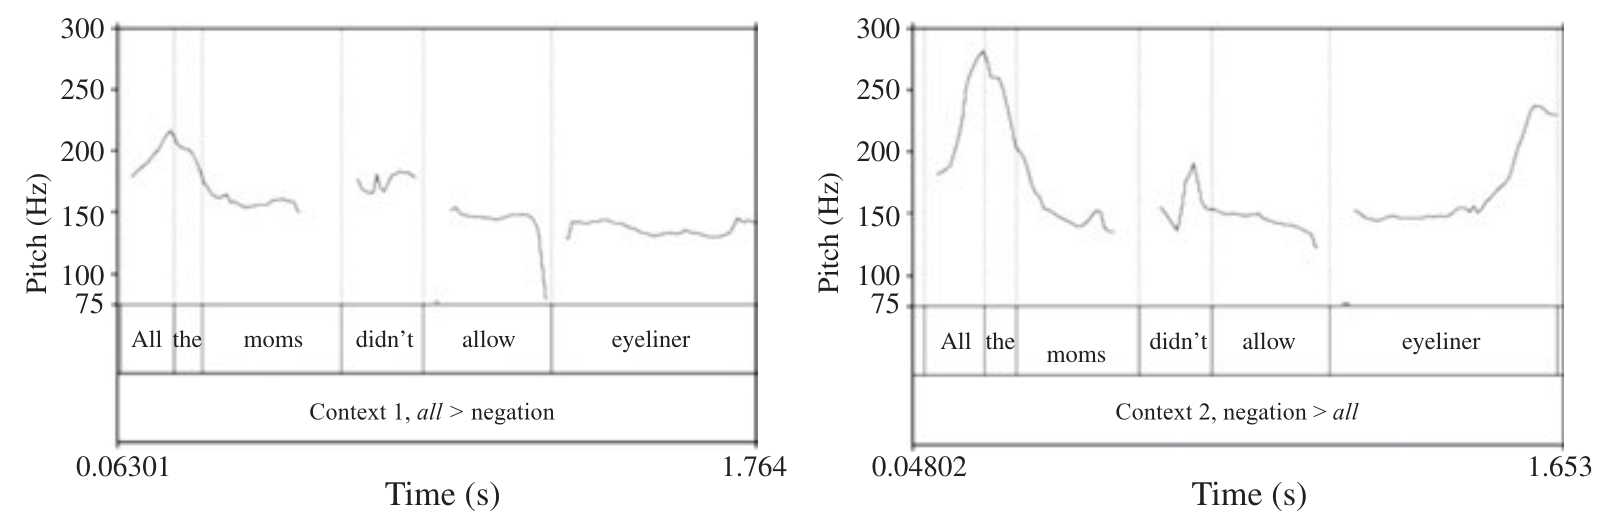
\includegraphics[width=\textwidth]{images/pitch 1.png}

\end{frame}

\begin{frame}
    \frametitle{Процесс}

    \begin{enumerate}
        \item (Участник тренируется на предложениях с двусмысленной местоименной референцией)
        \item Участник видит предложение
        \begin{itemize}
            \item[] \textit{All moms didn't allow eyeliner}
        \end{itemize}
        \item Участник слышит предложение в одной из интонаций
        \item Участник выбирает продолжение за 10 секунд
        \begin{itemize}
            \item[A.] \textit{They were all in agreement}
            \item[B.] \textit{Only the moms of the older girls let their daughters wear it}
        \end{itemize}
    \end{enumerate}

\end{frame}

\begin{frame}
    \frametitle{Результаты}

    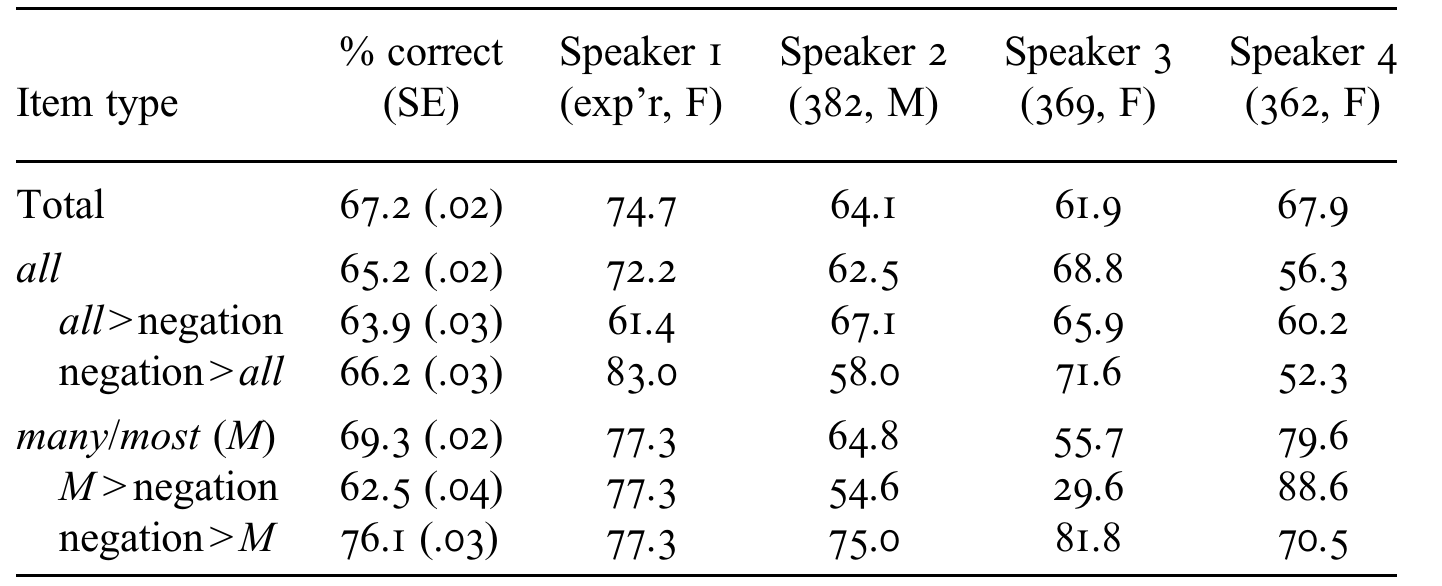
\includegraphics[width=\textwidth]{images/results 1.png}

    \only<1>{
        Результаты не ахти — но все-таки выше 50\%; ср. прежние исследования. Кроме того, филеры с neg/because дали сравнимые результаты.
    }

    \pause

    \begin{table}[stats]
        \centering
        \begin{tabular}{c | c c | c c}
            &                      S >$\neg$ & $\neg$ > all & DO >$\neg$ & $\neg$ > DO\\
            \hline
            BIN$_{p=.5, CI=99\%}$ & 2.7        & 3.1        & 2.5         & 5.1\\
            $p$                   & <.01       & .002       & .01         & <.0001\\
            \hline
            $\chi^2$              & (7) 20     & (7) 32     & (4) 21.45   & (4) 31.45\\
            $p$                   & <.01       & <.01       & <.01         & <.01\\
        \end{tabular}
        \label{<stats1>}
    \end{table}

\end{frame}

\begin{frame}
    \frametitle{Еще статистика}

    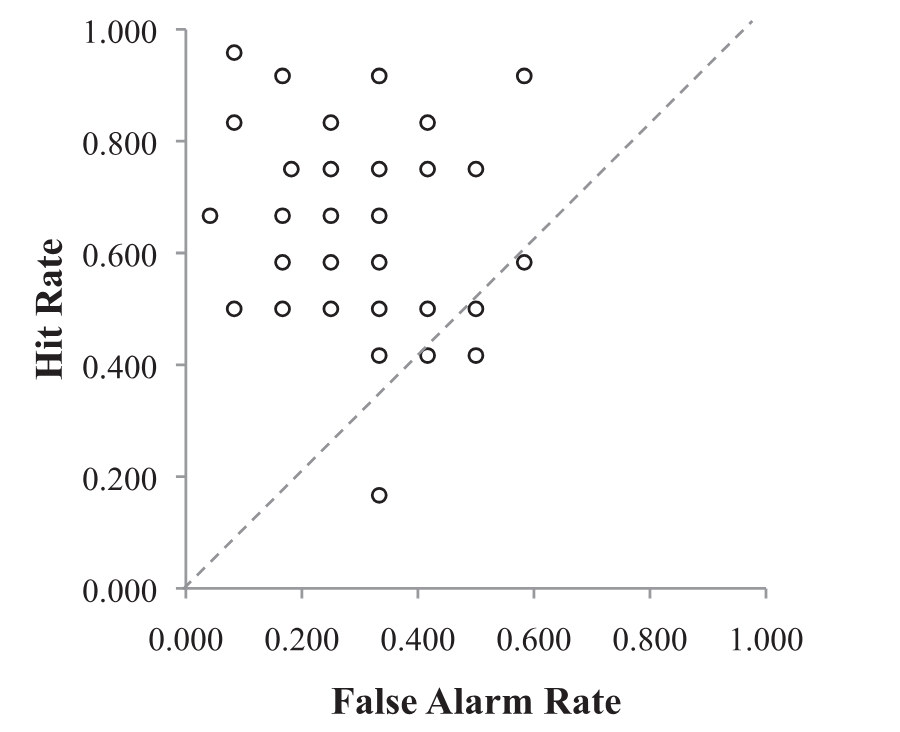
\includegraphics[width=20em]{images/hit n miss.png}

    $\overline{d'} = \overline{z(\text{Hits}) - z(\text{False alarms})} = 1.02$
    
    (от 0 до 4; авторы говорят, достаточно много.)

\end{frame}

\begin{frame}
    \frametitle{Что говорят участники?}

    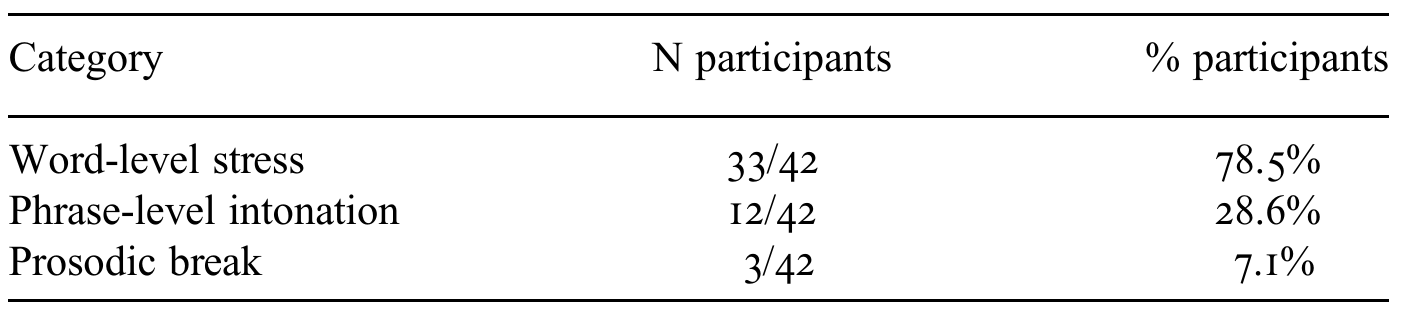
\includegraphics[width=\textwidth]{images/responses.png}

    \begin{itemize}
        \item Кажется, слушающие действительно опирались на задуманные говорящими просодические различия.
        \item Но на какие?
        \item Явно не на джекендорфовский финальный контур.
    \end{itemize}

\end{frame}

\subsection{Эксперимент 2: восприждение}

\begin{frame}
    \frametitle{Восприятие II}

    Может ли носитель определить относительную СД операторов по просодии?

    \begin{itemize}
        \item Может ли носитель выбрать более из двух интонаций более уместную в контексте?
    \end{itemize}

    Стимулы — аудиодорожки от наиболее «удачных» участников эксперимента на порождение (один мужчина, две женщины) и авторки с образованием вокалиста.

    (2 стимула с субъектным квантором + 1 с объектным) * (2 просодических контура) * (3 спикера\footnote{мужика убрали (почему — непонятно, вроде проблемы были с женщиной)}). Плюс столько же филеров.

    \pause

    37 андерградов.

\end{frame}

\begin{frame}
    \frametitle{Процесс}

    \begin{enumerate}
        \item (Участник тренируется на предложениях с двусмысленной местоименной референцией)
        \item Участник читает целый текст в самоскоростном режиме по предложениям
        \item Участник слушает два прочтения предложения
        \item Участник тыкает A или B (дольше 3.5 сек не считаем)
    \end{enumerate}

    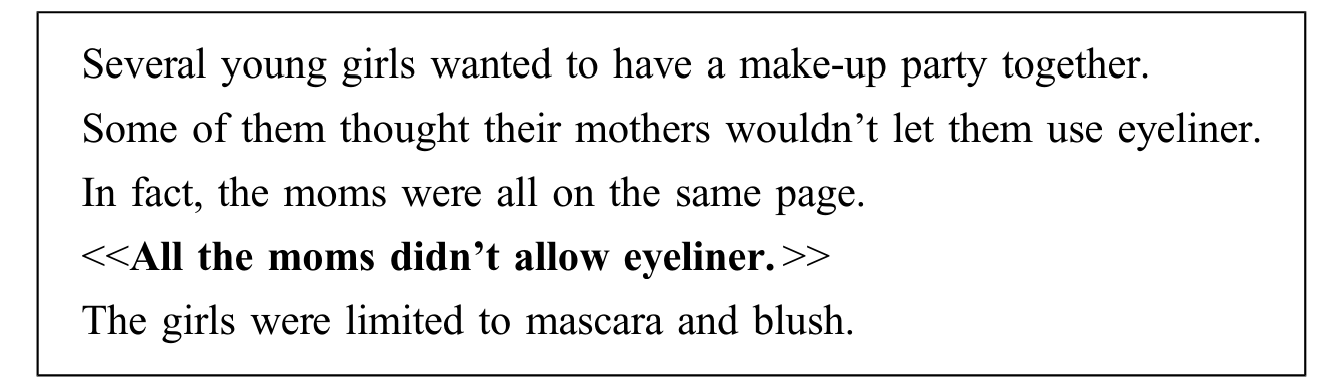
\includegraphics[width=\textwidth]{images/p2 ex.png}
\end{frame}

\begin{frame}
    \frametitle{Результаты}

    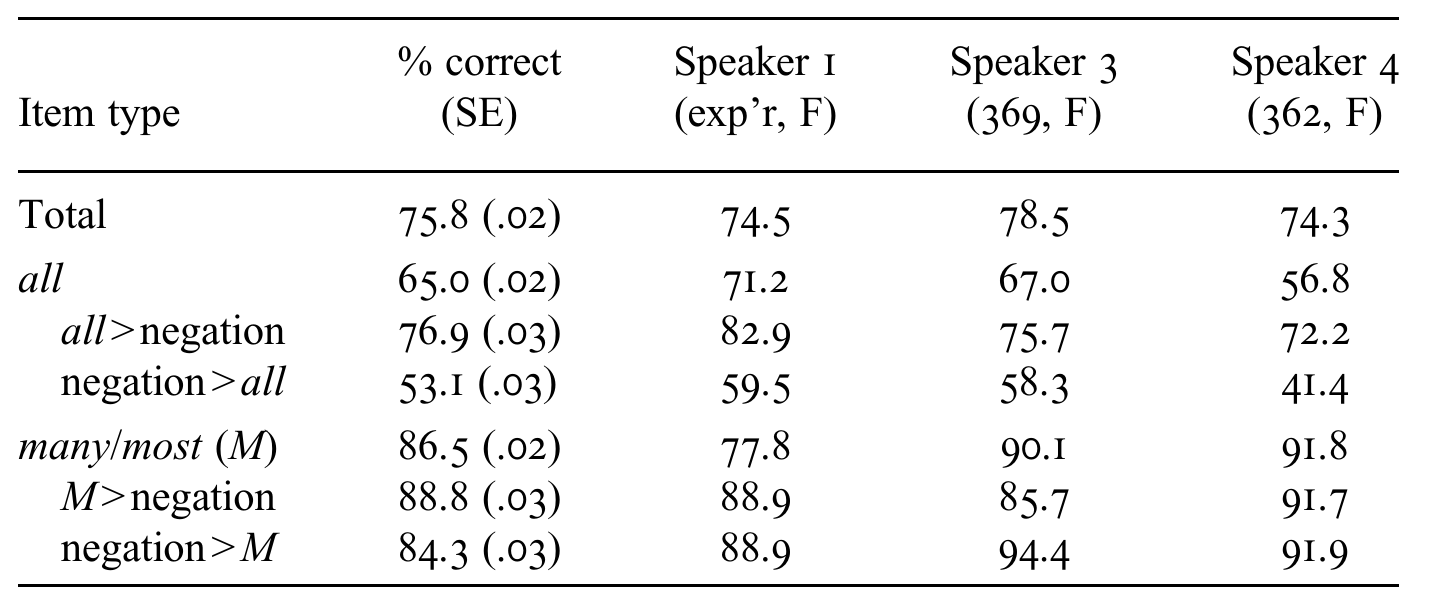
\includegraphics[width=\textwidth]{images/results 2.png}

    \only<1>{
        Совсем хорошие результаты (кроме $\neg$ > all). Результаты neg/because сравнимы.
    }

    \pause

    \begin{table}[stats]
        \centering
        \begin{tabular}{c | c c | c c}
            &                      S >$\neg$ & $\neg$ > all & DO >$\neg$ & $\neg$ > DO\\
            \hline
            BIN$_{p=.5, CI=99\%}$ & 5.0        & \textbf{-1.0}       & 27.4        & 6.5\\
            $p$                   & <.00001    & \textbf{.31}        & <.00001     & <.00001\\
            \hline
            $\chi^2$              & (6) 44.5   & (6) 23.33  & (3) 56.51   & (3) 43.54\\
            $p$                   & <.0001     &.0007       & <.0001      & <.0001\\
        \end{tabular}
        \label{<stats2>}
    \end{table}

\end{frame}

\begin{frame}
    \frametitle{Еще статистика}

    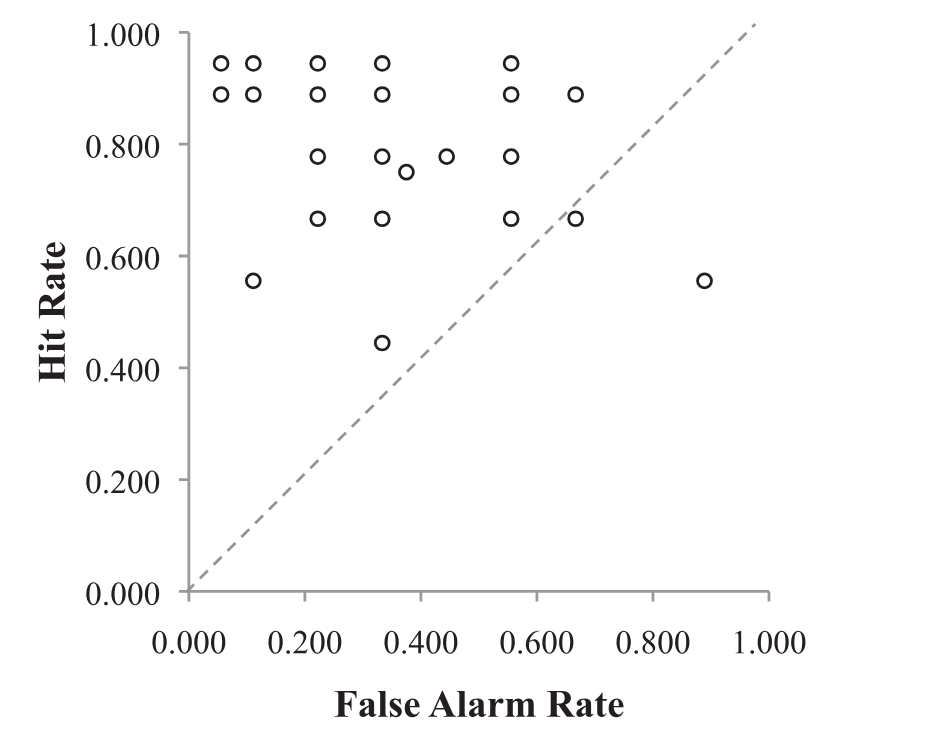
\includegraphics[width=20em]{images/hit n miss 2.png}

    $\overline{d'} = \overline{z(\text{Hits}) - z(\text{False alarms})} = 1.26$

\end{frame}

\begin{frame}
    \frametitle{Выводы}

    \begin{itemize}
        \item (судя по объектному) Носители хорошо чувствуют разницу и даже не предпочитают один контур другому\footnote{Насколько показателен в этом отношении forced choice?}.
        \pause
        \item В чем же проблема $\neg>$ all?
        \begin{itemize}
            \item Авторы: в том, что квантор предшествует отрицанию
            \pause
            \begin{itemize}
                \item Отрицание не с-командует квантором, так что это по умолчанию странная интерпретация (клаузальное отрицание? металингвистическое отрицание?).
                \item Квантор в просодически неудобной позиции (в начале предложения есть и другие требования к интонации)
                \item Последовательная обработка предложения не позволяет засунуть квантор под отрицание, потому что отрицания еще нет
            \end{itemize}
            \item Можно еще добавить: вапщета есть конкурирующее \textit{Not all the moms allowed eyeliner}
        \end{itemize}
        {\small N. B. Это все круто объясняет, почему RFR для $neg$ > DO должен обрабатываться лучше, чем для $neg$ > S. Но дело же не в этом. Обрабатывается-то хорошо, просто не порождается (вспомним э. 0).}
    \end{itemize}
\end{frame}

\end{document}
